% Standalone source: compile with pdfLaTeX twice on Overleaf.
% No external images, bibliography database, or shell escape are required.
\documentclass[11pt,a4paper]{article}
\usepackage[T1]{fontenc}
\usepackage[utf8]{inputenc}
\usepackage{lmodern}
\usepackage[margin=24mm,headheight=15pt]{geometry}
\usepackage{amsmath,amssymb,mathtools,bm}
\usepackage{microtype}
\usepackage{xcolor}
\usepackage{booktabs,tabularx,longtable,array}
\usepackage{enumitem}
\usepackage{tikz}
\usetikzlibrary{arrows.meta,calc}
\usepackage{fancyhdr}
\usepackage{hyperref}
\definecolor{ink}{HTML}{183B56}
\definecolor{accent}{HTML}{006D77}
\definecolor{warm}{HTML}{B05D25}
\hypersetup{colorlinks=true,linkcolor=ink,urlcolor=accent,
 pdftitle={Optics study notes through Section 4.4},
 pdfsubject={Eikonal, pupils, wavefront error, ray slopes, and paraboloidal mirrors}}
\pagestyle{fancy}
\fancyhf{}
\fancyhead[L]{\small Optics: phase, wavefronts, and ray error}
\fancyhead[R]{\small Study notes}
\fancyfoot[C]{\thepage}
\setlength{\parindent}{0pt}
\setlength{\parskip}{5pt}
\setlist{itemsep=2pt,topsep=4pt}
\allowdisplaybreaks[2]
\numberwithin{equation}{section}
\newcommand{\dd}{\mathrm{d}}
\newcommand{\ii}{\mathrm{i}}
\newcommand{\gradp}{\nabla_{\!\perp}}
\newcommand{\vct}[1]{\bm{#1}}
\newcommand{\avg}[1]{\left\langle #1\right\rangle}
\newcommand{\note}[1]{\par\smallskip\noindent{\color{accent}\textbf{Interpretation.}}\ #1\par\smallskip}
\newcommand{\caution}[1]{\par\smallskip\noindent{\color{warm}\textbf{Keep distinct.}}\ #1\par\smallskip}
\newcommand{\mm}{\,\mathrm{mm}}
\newcommand{\nm}{\,\mathrm{nm}}
\newcommand{\um}{\,\mu\mathrm{m}}
\newcolumntype{Y}{>{\raggedright\arraybackslash}X}

\begin{document}
\hypersetup{pageanchor=false}
{\color{ink}\Huge\bfseries Studying Aberrations from the Fundamentals}
\vspace{7mm}
\hypersetup{pageanchor=true}
\pagenumbering{roman}

\pagenumbering{arabic}

\section{Conventions and the mathematical tools}
\subsection{What is being described?}
A ray describes a direction and trajectory in geometrical optics. An
eikonal describes phase as a function of position. A surface sag describes
the physical shape of a lens or mirror. These are distinct quantities even
when some of them are measured in the same length units.

\begin{longtable}{@{}>{\raggedright\arraybackslash}p{.21\textwidth}>{\raggedright\arraybackslash}p{.55\textwidth}>{\raggedright\arraybackslash}p{.18\textwidth}@{}}
\toprule
Symbol & Meaning & Units\\ \midrule
\endhead
$\lambda_0,\ k_0=2\pi/\lambda_0$ & Vacuum wavelength and vacuum wavenumber & length; inverse length\\
$n,n'$ & Refractive indices; a prime labels the output medium & dimensionless\\
$\ell$ & Geometrical arc length along a ray & length\\
$\mathcal L=\int n\,\dd\ell$ & Optical path length & length\\
$S,\ W=S_{\rm a}-S_0$ & Eikonal; actual-minus-ideal wavefront error & length\\
$\vct r=(x,y,z)$ & Three-dimensional position & length\\
$r=\sqrt{x^2+y^2}$ & Radial pupil coordinate when the origin is on axis & length\\
$a,\ \rho=r/a$ & Physical pupil radius; normalized pupil radius & length; dimensionless\\
$u=x/a,\ v=y/a$ & Normalized Cartesian pupil coordinates & dimensionless\\
$\vct d=\dd\vct r/\dd\ell$ & Unit ray direction & dimensionless\\
$\vct q=(d_x,d_y)$ & Transverse direction cosines, not pupil position & dimensionless\\
$\vct s=(\dd x/\dd z,\dd y/\dd z)$ & Transverse ray slope & dimensionless\\
$L$ & Axial separation of comparison and image planes & length\\
$f$ & Focal length; it is not automatically equal to $L$ & length\\
\bottomrule
\end{longtable}

Unless a mirror example says otherwise, propagation is toward $+z$.
For transmitted systems a spherical radius is positive when its centre of
curvature lies downstream of the vertex. We use time dependence
$e^{-\ii\omega t}$ and real positive refractive indices. An \emph{exact} ray
formula is exact within geometrical optics, not an exact solution of the
electromagnetic diffraction problem.

\subsection{Units, derivatives, and coordinate normalization}
The conversions
\[
1\mm=10^{-3}\,\mathrm m,\qquad 1\um=10^{-3}\mm,\qquad
1\nm=10^{-6}\mm
\]
must be applied before combining wavelength, optical path, and geometry.
For example, $633\nm=0.000633\mm$. A path error $W$ produces phase error
\begin{equation}
 \Delta\phi=k_0W=\frac{2\pi W}{\lambda_0}.
\end{equation}
Thus $W=31.65\nm$ is $0.05$ waves at $633\nm$, giving
$\Delta\phi=0.31416$ radians. Angles in Taylor series are in radians:
$1^\circ=\pi/180$ radians.

For a sag $h(r)=cr^2/2$, the definition of derivative gives
\[
 \frac{h(r+\Delta r)-h(r)}{\Delta r}
 =cr+\frac{c\Delta r}{2}\longrightarrow cr.
\]
Hence $h'(r)=cr$ and $h''(r)=c$. A partial derivative varies one coordinate
while holding the others fixed. For example,
\begin{equation}
 W=A(x^2+y^2)^2
 \quad\Longrightarrow\quad
 \gradp W=4A(x^2+y^2)(x,y).
\end{equation}
If $W$ has units of length, $A$ here has units of inverse length cubed.
Writing the same function as $W=B\rho^4$ instead gives $B=Aa^4$,
which has units of length.

Define $\widetilde W(u,v)=W(au,av)$. The chain rule gives
\begin{equation}
 \frac{\partial W}{\partial x}
 =\frac1a\frac{\partial\widetilde W}{\partial u},
 \qquad
 \frac{\partial W}{\partial y}
 =\frac1a\frac{\partial\widetilde W}{\partial v},
 \qquad
 \gradp W=\frac1a\nabla_{u,v}\widetilde W.
 \label{eq:normalization}
\end{equation}
The normalized coordinates are dimensionless; $\widetilde W$ remains an
optical path in length units.

\subsection{Disk averages and wavefront statistics}
For $x=a\rho\cos\theta,\ y=a\rho\sin\theta$, a polar area element has
radial width $\dd r$ and tangential width $r\,\dd\theta$. Therefore
\[
 \dd A=r\,\dd r\,\dd\theta=a^2\rho\,\dd\rho\,\dd\theta,
 \qquad
 A_{\rm pupil}=\int_0^{2\pi}\int_0^1 a^2\rho\,\dd\rho\,\dd\theta=\pi a^2.
\]
Uniform full-disk area averaging means
\begin{equation}
 \avg{F}=\frac1\pi\int_0^{2\pi}\int_0^1
 F(\rho,\theta)\rho\,\dd\rho\,\dd\theta.
 \label{eq:average}
\end{equation}
For $m>-2$,
\begin{equation}
 \avg{\rho^m}=2\int_0^1\rho^{m+1}\,\dd\rho=\frac{2}{m+2}.
\end{equation}
In particular, $\avg{\rho^2}=1/2$, $\avg{\rho^4}=1/3$,
$\avg{\rho^6}=1/4$, and $\avg{\rho^8}=1/5$.

Expanding the square gives the piston-removed variance
\begin{equation}
 \sigma_W^2=\avg{(W-\avg W)^2}
 =\avg{W^2}-\avg W^2.
\end{equation}
For $W=B\rho^2$,
\[
 \avg W=B/2,\qquad
 \sigma_W^2=B^2\left(\frac13-\frac14\right)=\frac{B^2}{12},
 \qquad \sigma_W=\frac{|B|}{\sqrt{12}}.
\]
For comparison, $W=B\rho^4$ gives
$\sigma_W^2=B^2(1/5-1/9)=4B^2/45$. Both raw monomials have
peak-to-valley magnitude $|B|$, but different RMS values.
The weight $\rho$ is essential; uniform weighting in radius is a different
measurement from uniform weighting in pupil area.

\subsection{Taylor series, distance expansions, and matrix order}
Repeated differentiation of $f(\epsilon)=(1+\epsilon)^p$ gives
\[
 f^{(k)}(0)=p(p-1)\cdots(p-k+1).
\]
Inserting these derivatives into Taylor's formula yields
\[
 (1+\epsilon)^p
 =1+p\epsilon+\frac{p(p-1)}{2}\epsilon^2
 +\frac{p(p-1)(p-2)}6\epsilon^3+\cdots.
\]
The cases needed below include
\begin{align}
 \sqrt{1+\epsilon}
 &=1+\frac{\epsilon}{2}-\frac{\epsilon^2}{8}
 +\frac{\epsilon^3}{16}-\frac{5\epsilon^4}{128}+O(\epsilon^5),\\
 \sqrt{1-\epsilon}
 &=1-\frac{\epsilon}{2}-\frac{\epsilon^2}{8}
 -\frac{\epsilon^3}{16}-\frac{5\epsilon^4}{128}+O(\epsilon^5),\\
 (1+\epsilon)^{-1}&=1-\epsilon+\epsilon^2+O(\epsilon^3).
\end{align}
An $O(\epsilon^k)$ remainder is bounded in magnitude by a constant times
$|\epsilon|^k$ sufficiently near zero. It is not a global accuracy promise.

For $L>0$,
\begin{equation}
 \sqrt{L^2+r^2}
 =L+\frac{r^2}{2L}-\frac{r^4}{8L^3}
 +\frac{r^6}{16L^5}+O(r^8/L^7).
 \label{eq:distance-series}
\end{equation}
For a sphere opening toward $+z$, with positive radius magnitude $R$,
\begin{equation}
 h(r)=R-\sqrt{R^2-r^2}
 =\frac{r^2}{2R}+\frac{r^4}{8R^3}
 +\frac{r^6}{16R^5}+\frac{5r^8}{128R^7}+\cdots.
\end{equation}
The expansion parameters are $r^2/L^2$ and $r^2/R^2$, respectively.

For vectors, $\vct a\cdot\vct b=\sum_i a_i b_i$ and
$|\vct a|^2=\vct a\cdot\vct a$. A straight ray with unit direction
$\vct d$ is $\vct r(\ell)=\vct r_0+\ell\vct d$.
For matrices, if $M_1$ acts first and $M_2$ second, the result is
$M_2M_1\vct v$. This ordering matters when a translation and refraction
are composed.

\section{Optical path, phase, and the eikonal}
\subsection{From wavelength to optical path}
In a homogeneous transparent medium, the phase wavelength is
$\lambda=\lambda_0/n$. Travelling a geometrical distance $\dd\ell$ adds
\[
 \dd\phi=\frac{2\pi}{\lambda}\dd\ell=k_0 n\,\dd\ell.
\]
Summing along a ray gives
\begin{equation}
 \mathcal L=\int n\,\dd\ell,\qquad
 \phi=\phi_{\rm initial}+k_0\mathcal L.
 \label{eq:opl}
\end{equation}
For piecewise homogeneous media, $\mathcal L=\sum_jn_j\ell_j$.
Thus $10\mm$ of air followed by $5\mm$ of index $1.5$ has geometrical
length $15\mm$ and optical path $17.5\mm$.

\subsection{Eikonal means phase expressed as a length}
Write a monochromatic scalar field as
\begin{equation}
 U(\vct r,t)=A(\vct r)e^{\ii[k_0S(\vct r)-\omega t]}.
\end{equation}
The spatial phase is $k_0S$, so $S$ is phase measured in optical-length
units. Along a ray, \eqref{eq:opl} gives
\begin{equation}
 S(\vct r_2)-S(\vct r_1)=\int_{\vct r_1}^{\vct r_2}n\,\dd\ell.
 \label{eq:eikonal-integral}
\end{equation}
The integral follows the ray branch being described; its constant of
integration fixes the phase reference.

A wavefront is a surface $S(\vct r)=\text{constant}$ at fixed time.
If $\vct t$ is tangent to that surface, differentiation along it gives
$\nabla S\cdot\vct t=0$. Therefore $\nabla S$ is normal to the wavefront.

\subsection{Derive the eikonal equation from the scalar wave equation}
For the scalar approximation in an isotropic medium,
\[
 \nabla^2U+k_0^2n^2U=0.
\]
Substitute $U=Ae^{\ii k_0S}$. The first derivative is
\[
 \nabla U=e^{\ii k_0S}\left(\nabla A+\ii k_0A\nabla S\right).
\]
Taking the divergence and using the product rule,
\begin{align}
 \nabla^2U=e^{\ii k_0S}\big[
 \nabla^2A+2\ii k_0\nabla A\cdot\nabla S
 +\ii k_0A\nabla^2S-k_0^2A|\nabla S|^2\big].
\end{align}
After substitution and cancellation of the exponential,
\begin{equation}
 \nabla^2A+2\ii k_0\nabla A\cdot\nabla S+\ii k_0A\nabla^2S
 +k_0^2A(n^2-|\nabla S|^2)=0.
\end{equation}
When wavelength is short compared with the amplitude and material variation
scales, the leading $k_0^2$ terms must cancel:
\begin{equation}
 \boxed{|\nabla S|^2=n^2.}
 \label{eq:eikonal}
\end{equation}
Locally the phase is
$k_0S(\vct r_0)+k_0\nabla S(\vct r_0)\cdot\Delta\vct r$.
It is a local plane wave with wavevector $\vct k=k_0\nabla S$.
In an isotropic medium its ray direction is along $\vct k$, giving
\begin{equation}
 \boxed{\vct d=\frac{\nabla S}{n}.}
 \label{eq:ray-eikonal}
\end{equation}
This reproduces textbook Eq.~(2.6).
The slowly varying amplitude and single-ray-branch assumptions need care at
caustics, near sharp boundaries, and where diffraction is essential.

\subsection{Why equal phase at a target is the ideal focusing condition}
At pupil point $Q$, the initial phase is $k_0S(Q)$.
The scalar geometrical propagation phase to a target $F$ adds
$k_0n'|F-Q|$. For contributions with amplitudes $a_j\geq0$, the field at $F$
has the form
\[
 U(F)=\sum_j a_j e^{\ii k_0[S(Q_j)+n'|F-Q_j|]}.
\]
For two terms,
\[
 |a_1e^{\ii\phi_1}+a_2e^{\ii\phi_2}|^2
 =a_1^2+a_2^2+2a_1a_2\cos(\phi_1-\phi_2).
\]
For fixed amplitudes this is largest when their phases agree modulo $2\pi$.
For the whole pupil, $|U(F)|\leq\sum_j a_j$, with equality when all
nonzero phasors align. The ideal smooth coherent reference therefore obeys
\begin{equation}
 \boxed{S_{\rm ideal}(Q)+n'|F-Q|=C.}
 \label{eq:constant-focus}
\end{equation}
Strictly, equality modulo $\lambda_0$ suffices for the optical lengths.
On a connected pupil with a smooth unwrapped eikonal, the integer-wavelength
offset is constant and can be absorbed into $C$.

There is also a ray proof. For $Q=(x,y,0)$ and $F=(0,0,L)$, the desired
ray direction is $(-x,-y,L)/\sqrt{L^2+r^2}$. Hence
$S_x=-n'x/\sqrt{L^2+r^2}$ and $S_y=-n'y/\sqrt{L^2+r^2}$.
Since the distance derivatives are $x/\sqrt{L^2+r^2}$ and
$y/\sqrt{L^2+r^2}$,
$\gradp(S+n'\sqrt{L^2+r^2})=0$. This is exactly
\eqref{eq:constant-focus}.

\note{An outer pupil point has a longer remaining distance. An ideal
focusing wave has a starting phase that compensates that difference.
Different remaining distances do not by themselves imply aberration.
An ideal focus is an unaberrated coherent reference; a finite aperture
still produces a diffraction pattern of finite width.}

\section{Reflection and refraction from optical path}
\subsection{Fermat's principle and Snell's law}
Fermat's principle states that the optical path is stationary under allowed
small path variations with the endpoints fixed. Stationary means zero first
variation; it does not necessarily mean a global minimum.

Put an interface at $z=0$, a source at $A=(x_A,-h_1)$ in index $n_1$,
and a destination at $B=(x_B,h_2)$ in index $n_2$. A trial crossing point
is $P=(x,0)$, so
\[
 \mathcal L(x)
 =n_1\sqrt{(x-x_A)^2+h_1^2}
 +n_2\sqrt{(x_B-x)^2+h_2^2}.
\]
Differentiate each square root:
\[
 \frac{\dd\mathcal L}{\dd x}
 =n_1\frac{x-x_A}{\sqrt{(x-x_A)^2+h_1^2}}
 -n_2\frac{x_B-x}{\sqrt{(x_B-x)^2+h_2^2}}.
\]
The ratios are the signed sines of the incident and transmitted angles
measured from the normal. Stationarity therefore gives
\begin{equation}
 \boxed{n_1\sin i=n_2\sin t.}
\end{equation}
For reflection, both endpoints are in the same medium and the two path
segments lie on the same side of the surface. The corresponding stationary
condition preserves the tangential direction component while the normal
component reverses.

\subsection{Exact vector reflection}
Let $\vct N$ be either unit normal at the reflecting point. Decompose an
incident unit direction into
\[
 \vct d_{\rm n}=(\vct d_{\rm in}\cdot\vct N)\vct N,\qquad
 \vct d_{\rm t}=\vct d_{\rm in}-\vct d_{\rm n}.
\]
Specular reflection preserves $\vct d_{\rm t}$ and reverses
$\vct d_{\rm n}$, hence
\begin{equation}
 \boxed{
 \vct d_{\rm out}
 =\vct d_{\rm in}-2(\vct d_{\rm in}\cdot\vct N)\vct N.
 }
 \label{eq:reflection}
\end{equation}
Changing $\vct N$ to $-\vct N$ leaves this expression unchanged.
Its norm is one because the orthogonal tangential and normal components
retain their respective squared magnitudes. At normal incidence,
$(0,0,-1)$ becomes $(0,0,1)$.

\subsection{Exact vector refraction and total internal reflection}
Choose $\vct N$ to point into the incident medium, so
$\vct d_{\rm in}\cdot\vct N<0$. Define
\[
 \eta=\frac{n_1}{n_2},\qquad c_i=-\vct d_{\rm in}\cdot\vct N.
\]
The incident tangential vector is $\vct d_{\rm in}+c_i\vct N$.
Snell's law scales it by $\eta$. Unit normalization determines the
transmitted normal magnitude:
\[
 c_t^2=1-\eta^2|\vct d_{\rm in}+c_i\vct N|^2
 =1-\eta^2(1-c_i^2).
\]
The transmitted ray points away from the incident medium, so its normal
component is $-c_t\vct N$. Therefore
\begin{equation}
 \boxed{
 c_t=\sqrt{1-\eta^2(1-c_i^2)},\qquad
 \vct d_{\rm tr}
 =\eta\vct d_{\rm in}+(\eta c_i-c_t)\vct N.
 }
\end{equation}
If the square root is imaginary, there is no propagating transmitted ray
in this model. For $n_1>n_2$, the threshold is
\[
 \sin i_c=\frac{n_2}{n_1}.
\]
For $n_1=1.5$ and $n_2=1$, $i_c\simeq41.81^\circ$.
At normal incidence $\vct d_{\rm in}=-\vct N$ and the formula returns
$\vct d_{\rm tr}=-\vct N$, as it should.

\section{First-order imaging: surfaces, lenses, and mirrors}
\subsection{Paraxial power of a spherical refracting surface}
In a meridional section, let the ray height be $y$ and its signed angle
to $+z$ be $\vartheta$. Near the axis,
\[
 \sin\vartheta\simeq\vartheta,\qquad
 \tan\vartheta\simeq\vartheta,\qquad \cos\vartheta\simeq1.
\]
These approximations retain only first-degree terms in heights and angles.

A spherical surface of signed radius $R$ has sag
$h(y)\simeq y^2/(2R)$ and normal angle $\alpha_N\simeq-y/R$.
Linearizing Snell's law about that normal gives
\[
 n(\vartheta-\alpha_N)=n'(\vartheta'-\alpha_N).
\]
Rearranging,
\begin{equation}
 \boxed{
 n'\vartheta'=n\vartheta-\frac{n'-n}{R}y.
 }
 \label{eq:surface-power}
\end{equation}
Define the surface power $\Phi=(n'-n)/R$ and reduced angle $p=n\vartheta$.
The refraction law becomes $p'=p-\Phi y$.

For an on-axis real object a distance $s_o>0$ before the surface and real
image a distance $s_i>0$ after it,
$\vartheta\simeq y/s_o$ and $\vartheta'\simeq-y/s_i$. Substitution gives
\begin{equation}
 \boxed{\frac{n}{s_o}+\frac{n'}{s_i}=\frac{n'-n}{R}.}
\end{equation}
The real conjugate distances use the indicated positive convention;
virtual conjugates acquire negative values in this formula.

\subsection{Thin-lens equation from rays and from optical path}
For a thin lens of glass index $n_g$ surrounded by air, add the powers
of its two surfaces:
\begin{equation}
 \Phi=(n_g-1)\left(\frac1{R_1}-\frac1{R_2}\right),\qquad
 \vartheta_{\rm out}=\vartheta_{\rm in}-\Phi y.
\end{equation}
For collimated input $\vartheta_{\rm in}=0$, the ray reaches the axis
after distance $f$ when $y+f(-\Phi y)=0$. Thus
\begin{equation}
 \boxed{\frac1f=(n_g-1)\left(\frac1{R_1}-\frac1{R_2}\right).}
\end{equation}
For finite conjugates, $\vartheta_{\rm in}=y/s_o$ and
$\vartheta_{\rm out}=-y/s_i$, giving
\begin{equation}
 \boxed{\frac1{s_o}+\frac1{s_i}=\frac1f,\qquad
 m=\frac{y_i}{y_o}=-\frac{s_i}{s_o}.}
\end{equation}
The magnification follows by tracing the central paraxial ray.

For an independent phase derivation, the change in biconvex thickness is
\[
 t(y)-t(0)\simeq\frac{y^2}{2}\left(\frac1{R_2}-\frac1{R_1}\right).
\]
Between fixed planes, replacing air by glass adds
$(n_g-1)[t(y)-t(0)]=-y^2/(2f)$. The paths from the object and to the image
add $y^2/(2s_o)$ and $y^2/(2s_i)$ to quadratic order. Equal phase requires
\[
 \frac{y^2}{2}\left(\frac1{s_o}+\frac1{s_i}-\frac1f\right)=0,
\]
reproducing the ray result.

For $n_g=1.5$, $R_1=50\mm$, and $R_2=-50\mm$, $f=50\mm$.
An object at $s_o=200\mm$ has $s_i=66.6667\mm$ and $m=-1/3$.

\caution{The thickness-only calculation is sufficient here at Gaussian
order. Extending it to high powers does not automatically give the exact
aberration of a real lens: internal ray bending, oblique glass paths, and
different intersection heights also contribute.}

\subsection{Paraxial focal length and imaging law of a spherical mirror}
For this mirror only, use incident light along $-z$ and reflected light
toward $+z$. The surface opens toward $+z$:
\[
 h(r)=R-\sqrt{R^2-r^2}\simeq\frac{r^2}{2R}.
\]
In a meridional section its unit normal is approximately
$\vct N=(-r/R,0,1)$ to first order. Applying \eqref{eq:reflection} to
$\vct d_{\rm in}=(0,0,-1)$ gives
$\vct d_{\rm out}\simeq(-2r/R,0,1)$.
The ray height after axial distance $f$ is approximately
$r-2fr/R$, so
\begin{equation}
 \boxed{f=\frac R2.}
\end{equation}

For finite positive object and image distances $s_o,s_i$ in front of this
mirror, the geometrical path via radius $r$ is
\[
 \sqrt{r^2+[s_o-h(r)]^2}+\sqrt{r^2+[s_i-h(r)]^2}.
\]
For either conjugate $s$,
\[
 \sqrt{r^2+[s-h(r)]^2}
 =s-h(r)+\frac{r^2}{2s}+O(r^4)
 =s+r^2\left(\frac1{2s}-\frac1{2R}\right)+O(r^4).
\]
Summing and setting the quadratic coefficient to zero gives
\begin{equation}
 \boxed{\frac1{s_o}+\frac1{s_i}=\frac2R=\frac1f.}
\end{equation}
The omitted terms generally prevent a sphere from focusing all
finite-aperture rays at one point. The paraboloid at the end provides an
exact on-axis counterexample: it focuses an axial plane wave without
geometrical spherical aberration.

\subsection{Matrices, thick lenses, principal planes, and invariants}
Use the ray vector $(y,p)^{\mathsf T}$ with $p=n\vartheta$.
Translation by distance $d$ in index $n$ gives
$y'=y+(d/n)p$ and $p'=p$. A refracting surface preserves height and
changes $p$ to $p-\Phi y$. Their matrices are
\begin{equation}
 T(d,n)=\begin{pmatrix}1&d/n\\0&1\end{pmatrix},\qquad
 R(\Phi)=\begin{pmatrix}1&0\\-\Phi&1\end{pmatrix}.
\end{equation}
For a lens of thickness $d$ and index $n_g$,
\begin{align}
 M&=R(\Phi_2)T(d,n_g)R(\Phi_1)\\
 &=R(\Phi_2)
 \begin{pmatrix}1-d\Phi_1/n_g&d/n_g\\-\Phi_1&1\end{pmatrix}\\
 &=\begin{pmatrix}
 1-d\Phi_1/n_g&d/n_g\\
 -\Phi_1-\Phi_2+d\Phi_1\Phi_2/n_g&1-d\Phi_2/n_g
 \end{pmatrix}
 =\begin{pmatrix}A&B\\C&D\end{pmatrix}.
\end{align}
The effective power is $\Phi_{\rm eff}=-C$.
For air on both sides, the effective focal length is
$f_{\rm EFL}=-1/C$. A collimated ray $(y_0,0)$ exits as
$(Ay_0,Cy_0)$. After a further air distance $b$, its height is
$(A+bC)y_0$, giving
\begin{equation}
 \boxed{f_{\rm EFL}=-\frac1C,\qquad \mathrm{BFL}=-\frac AC.}
\end{equation}
BFL is measured from the rear vertex. EFL is measured from the rear
principal plane, the effective reference plane for first-order focusing.

For the preceding biconvex lens with $d=5\mm$,
$\Phi_1=\Phi_2=0.01\,\mathrm{mm}^{-1}$ and
\[
 A=D=\frac{29}{30},\qquad B=\frac{10}{3}\mm,\qquad
 C=-\frac{59}{3000}\,\mathrm{mm}^{-1}.
\]
Thus $f_{\rm EFL}=3000/59=50.84746\mm$ and
$\mathrm{BFL}=2900/59=49.15254\mm$.
If the first vertex is $z=0$, the paraxial image of an axial plane wave is
at $z=5+\mathrm{BFL}=54.15254\mm$.

Include the object-to-system and system-to-image translations in a total
matrix. Then $y_i=Ay_o+Bp_o$. All rays from the same object point have
fixed $y_o$ and variable $p_o$, so the imaging condition is
\begin{equation}
 \boxed{B=0,\qquad y_i=Ay_o.}
\end{equation}
Both elementary matrices have determinant one, giving $AD-BC=1$.
For two rays,
\begin{align}
 y'_1p'_2-y'_2p'_1
 &=(Ay_1+Bp_1)(Cy_2+Dp_2)
 -(Ay_2+Bp_2)(Cy_1+Dp_1)\\
 &=(AD-BC)(y_1p_2-y_2p_1)=y_1p_2-y_2p_1.
\end{align}
This preserved combination is a useful first-order consistency check.

\section{Pupils and reference wavefronts}
\subsection{Pupil position selects a ray; field position selects an object point}
For a fixed object point, the aperture stop limits the admitted ray cone.
It can be an iris, lens rim, or mirror boundary. The entrance pupil is its
image through the preceding optics, seen from object space; the exit pupil
is its image through the following optics, seen from image space. Either
pupil can be virtual and neither must coincide with a physical lens surface.

A chief ray passes through the stop centre. A marginal ray passes through
its edge. A field stop limits admitted object positions. Vignetting clips
some field bundles and changes the pupil shape or weighting.

\begin{center}
\begin{tabularx}{\textwidth}{@{}lY@{}}
\toprule
Change & What it selects\\ \midrule
Change pupil coordinate & A different ray from the same object point\\
Change field coordinate & A different object point or incident field angle\\
Change reference image & A different target against which those rays are judged\\
\bottomrule
\end{tabularx}
\end{center}

For an object at infinity in air, the f-number is
$N=f_{\rm EFL}/D_{\rm entrance}$.
The image-space numerical aperture is $\mathrm{NA}=n'\sin\alpha$.
If the relevant pupil radius is $a$, its axial distance to focus is $L$,
and the cone is paraxial, $\tan\alpha=a/L$ gives
$\mathrm{NA}\simeq n'a/L$.
When additionally $L\simeq f_{\rm EFL}$, the relevant diameter is
$2a=D_{\rm entrance}$, and $n'=1$, this becomes
$\mathrm{NA}\simeq1/(2N)$. The shortcut is not general at finite conjugates
or large aperture.

\subsection{Specify the ideal before defining the error}
Let the comparison plane be $z=z_e$ and the reference image be
$F=(X_0,Y_0,z_f)$, with $L=z_f-z_e>0$.
Equation \eqref{eq:constant-focus} gives textbook Eq.~(4.1):
\begin{equation}
 S_0(x,y)=C-n'\sqrt{(x-X_0)^2+(y-Y_0)^2+L^2}.
 \label{eq:ideal}
\end{equation}
The sign is fixed by convergence:
\[
 \frac{\partial S_0}{\partial x}
 =-\frac{n'(x-X_0)}
 {\sqrt{(x-X_0)^2+(y-Y_0)^2+L^2}},
\]
whose direction component points toward $X_0$.
The wavefront error is textbook Eq.~(4.2):
\begin{equation}
 \boxed{W(x,y)=S_{\rm a}(x,y)-S_0(x,y).}
 \label{eq:opd}
\end{equation}
Equivalently, $W(Q)=S_{\rm a}(Q)+n'|F-Q|-C$.
The segment from $Q$ to $F$ defines the subtracted ideal. An aberrated
physical ray is not thereby forced to pass through $F$.

\note{An ideal wave can have nonzero slope and curvature while $W=0$.
At an off-centre pupil point its ray is inclined toward the image, but it
has no directional error relative to the ideal ray at that same point.
The word error describes a mismatch with the specified reference.}

\subsection{Piston: constant phase across the pupil}
For $W=P$, the phase multiplier is $e^{\ii k_0P}$.
Every contribution to a coherent image receives the same factor, so
\[
 U_{\rm new}=e^{\ii k_0P}U_{\rm old},\qquad
 |U_{\rm new}|^2=|U_{\rm old}|^2,\qquad \gradp P=0.
\]
Piston changes neither ray directions nor the intensity of that isolated
coherent image. Differential piston between coherent interferometer arms or
mirror segments can change interference.

With a specified pupil weight, mean-piston removal is
\[
 P_{\rm mean}=\avg W,\qquad W_{\rm residual}=W-\avg W.
\]
Setting $W(0)=0$ is a different reference choice. For example,
$W=B\rho^2$ has zero centre value but nonzero mean $B/2$.
On the uniformly weighted full disk, mean removal gives
$B(\rho^2-1/2)$. A constant Taylor coefficient and the fitted full-pupil
piston need not be numerically equal.

\subsection{Where linear terms come from: tilt relative to the reference}
A smooth pupil function can be Taylor-expanded:
\begin{align}
 W(x,y)={}&W(0)+W_x(0)x+W_y(0)y\\
 &+\frac12\left[W_{xx}(0)x^2+2W_{xy}(0)xy+W_{yy}(0)y^2\right]+\cdots.
\end{align}
The linear terms are present when the reference and actual directions
differ at the expansion point; they are not created by merely choosing
an off-centre pupil point.

For a plane wave in homogeneous index $n'$,
$\vct k=n'k_0\vct d$ and
$U=Ae^{\ii(\vct k\cdot\vct r+\phi_a)}$. Comparing with $Ae^{\ii k_0S}$
gives
\[
 S_{\rm a}(\vct r)=n'\vct d\cdot\vct r+C_a.
\]
On $z=0$ this is $n'd_xx+n'd_yy+C_a$. The axial reference plane wave has
$S_0=n'z+C_r$, which is constant only across a fixed $z$ plane.
Subtracting on $z=0$ yields
\begin{equation}
 \boxed{
 W=P+b_xx+b_yy,\qquad b_x=n'd_x,\quad b_y=n'd_y.
 }
\end{equation}
For an inclination $\alpha$ in the $xz$ plane,
$W=P+n'x\sin\alpha\simeq P+n'\alpha x$.
Its gradient is constant. Section~\ref{sec:rayerror} will show that this
produces a uniform image shift paraxially.

\subsection{Quadratic radial error and a shifted reference focus}
For an axial focus, use \eqref{eq:distance-series} in \eqref{eq:ideal}:
\begin{equation}
 S_0(r;L)=P(L)-\frac{n'r^2}{2L}+\frac{n'r^4}{8L^3}
 -\frac{n'r^6}{16L^5}+\cdots.
\end{equation}
The quadratic term in $S_0$ is required for ideal convergence. A radial
quadratic term in the \emph{difference} $W$ is defocus.

Hold $S_{\rm a}$ fixed on the same comparison plane and replace the target
distance $L$ by $L+\Delta L$. Then
\begin{align}
 W_{\rm new}-W_{\rm old}
 &=S_0(r;L)-S_0(r;L+\Delta L)\\
 &=\Delta P+\frac{n'r^2}{2}
 \left(\frac1{L+\Delta L}-\frac1L\right)
 -\frac{n'r^4}{8}
 \left(\frac1{(L+\Delta L)^3}-\frac1{L^3}\right)+\cdots.
\end{align}
The reciprocal difference is
$-\Delta L/[L(L+\Delta L)]\simeq-\Delta L/L^2$
when $|\Delta L|\ll L$. Therefore textbook Eq.~(4.3) is
\begin{equation}
 \boxed{
 W_{\rm new}=W_{\rm old}-\frac{n'\Delta L}{2L^2}r^2
 +\text{piston}+\text{higher-order terms}.
 }
 \label{eq:refocus}
\end{equation}
The next term, first order in $\Delta L$, is
$3n'\Delta L\,r^4/(8L^4)$.
Both a small pupil angle $r/L$ and a small relative shift $\Delta L/L$
have been used.

For an exact check, choose the on-axis reference values of both ideal
eikonals to be zero. Then
\[
 W_{\rm new}-W_{\rm old}
 =n'\left[
 \sqrt{(L+\Delta L)^2+r^2}
 -\sqrt{L^2+r^2}-\Delta L
 \right].
\]
Differentiating at $\Delta L=0$ gives
$n'[L/\sqrt{L^2+r^2}-1]\Delta L$.
Its small-$r/L$ expansion reproduces the negative quadratic coefficient.

For $\Delta L>0$, the new ideal wave converges less strongly and its
quadratic eikonal is less negative. Subtracting it makes the error more
negative away from the centre. If the unchanged actual rays focus at $L$,
a ray starting at $x$ follows $x(z)=x(1-z/L)$ and reaches the new plane at
$x(L+\Delta L)=-x\Delta L/L$. This is defocus at the displaced plane,
even though the actual focus has not moved.

With $\rho=r/a$ and $W=B\rho^2$, \eqref{eq:refocus} gives
\begin{equation}
 \boxed{\Delta B=-\frac{n'a^2\Delta L}{2L^2}.}
\end{equation}
For $n'=1$, $a=10\mm$, $L=200\mm$, and $\Delta L=0.1\mm$,
$\Delta B=-0.000125\mm=-125\nm$.
This is the change in edge-minus-centre quadratic OPD.

\subsection{Reference changes, physical changes, and general quadratic terms}
A reference change gives $\Delta W=-\Delta S_0$ at fixed actual wave.
A physical change gives $\Delta W=+\Delta S_{\rm a}$ at fixed reference.
For example, adding $g r^2$ to the physical eikonal adds phase $k_0gr^2$
and changes the actual convergence according to
\[
 -\frac{n'r^2}{2L}+gr^2
 =-\frac{n'r^2}{2}\left(\frac1L-\frac{2g}{n'}\right).
\]
As long as it remains converging, its new paraxial focus satisfies
$1/L_{\rm a,new}=1/L-2g/n'$. A small positive $g$ moves that physical
focus farther away.

For an actual perfect focus at $L_a$ and reference at $L$,
\[
 W(r)\simeq P+\frac{n'}2\left(\frac1L-\frac1{L_a}\right)r^2.
\]
It vanishes apart from piston when $L_a=L$.
Finally, an arbitrary quadratic form is
\[
 A x^2+2Bxy+C y^2
 =\frac{A+C}{2}(x^2+y^2)
 +\frac{A-C}{2}(x^2-y^2)+2Bxy.
\]
Only the rotationally symmetric first term is pure radial defocus. The
remaining terms represent unequal directional curvature. Linear/quadratic
here refers to pupil powers, not to the separate Seidel order convention.

\section{From wavefront slope to ray error: complete Section 4.4}
\label{sec:rayerror}
\subsection{Specify the two rays and the error being measured}
Set the output comparison plane to $z=0$ and the image plane to $z=L$.
Write $\vct\xi=(x,y)$ for a physical transverse position on the output
plane. The actual and ideal rays start at this same point and have unit
directions $\vct d$ and $\vct d_0$.
Define the transverse ray-intercept error
\begin{equation}
 \Delta\vct\xi=\vct\xi_{\rm image,a}-\vct\xi_{\rm image,0}.
\end{equation}
It is measured across the image plane, in length units. A uniform
displacement shifts a point image; varying displacements across the pupil
produce a geometrical blur. No numerical mistake is implied by the word
error.

\subsection{Wavefront gradient gives a direction-cosine difference}
Apply \eqref{eq:ray-eikonal} to each wave in the same output index $n'$:
\[
 \vct q=\frac{\gradp S_{\rm a}}{n'},\qquad
 \vct q_0=\frac{\gradp S_0}{n'}.
\]
Subtracting and using \eqref{eq:opd},
\begin{equation}
 \boxed{
 \delta\vct q=\vct q-\vct q_0=\frac{\gradp W}{n'}.
 }
 \label{eq:dq}
\end{equation}
This is an exact difference within the eikonal model on the stated plane.
Here $\delta\vct q$ denotes the finite difference; it need not yet be
linearized.

\subsection{Direction and slope use different independent distances}
Since $\ell$ is geometrical arc length, the full unit direction is
\[
 \vct d=\frac{\dd\vct r}{\dd\ell},\qquad
 \vct q=\left(\frac{\dd x}{\dd\ell},\frac{\dd y}{\dd\ell}\right).
\]
The axial coordinate $z$ is generally not the distance travelled along
the inclined ray. By the chain rule,
\[
 \frac{\dd x}{\dd z}
 =\frac{\dd x/\dd\ell}{\dd z/\dd\ell}
 =\frac{d_x}{d_z},\qquad
 \frac{\dd y}{\dd z}=\frac{d_y}{d_z}.
\]
For the forward branch,
$d_z=\sqrt{1-|\vct q|^2}>0$. Therefore
\begin{equation}
 \boxed{
 \vct s(\vct q)=\frac{\vct q}{\sqrt{1-|\vct q|^2}}.
 }
 \label{eq:slope}
\end{equation}
In a meridional plane, $q_x=\sin\alpha$, $d_z=\cos\alpha$, and
$s_x=\tan\alpha$.
The slope is dimensionless; at finite angle it is not the angle in radians.

\subsection{Exact propagation and textbook Eq.~(4.5)}
The actual ray is
$\vct R(\ell)=(x,y,0)+\ell\vct d$.
At the image plane, $\ell d_z=L$, giving
\[
 \vct\xi_{\rm image,a}=\vct\xi+L\frac{\vct q}{d_z}
 =\vct\xi+L\vct s(\vct q).
\]
The ideal ray similarly gives
$\vct\xi_{\rm image,0}=\vct\xi+L\vct s(\vct q_0)$.
Subtracting cancels the common starting position:
\begin{equation}
 \boxed{
 \Delta\vct\xi
 =L\left[
 \vct s\left(\vct q_0+\frac{\gradp W}{n'}\right)
 -\vct s(\vct q_0)
 \right].
 }
 \label{eq:exact-intercept}
\end{equation}
This is textbook Eq.~(4.5). The two directions must both be forward
propagating, so $|\vct q_0|<1$ and
$|\vct q_0+\gradp W/n'|<1$.

For reference image $F=(X_0,Y_0,L)$, let
$R_0=\sqrt{L^2+|\vct\xi-F_\perp|^2}$. Then
\[
 \vct q_0=\frac{F_\perp-\vct\xi}{R_0},\qquad
 d_{0z}=\frac L{R_0},\qquad
 \vct s(\vct q_0)=\frac{F_\perp-\vct\xi}{L}.
\]
Consequently $\vct\xi+L\vct s(\vct q_0)=F_\perp$ exactly, providing a
direct reference-geometry check.

\subsection{Paraxial propagation, the sign, and normalized coordinates}
If both directions are close to $+z$, then $d_z\simeq d_{0z}\simeq1$
and $\vct s(\vct q)\simeq\vct q$. Equation
\eqref{eq:exact-intercept} becomes textbook Eq.~(4.4):
\begin{equation}
 \boxed{
 \Delta\vct\xi\simeq\frac{L}{n'}\gradp W.
 }
 \label{eq:parax-intercept}
\end{equation}
The sign is positive because both errors are actual minus ideal.
For example, $W_x>0$ adds a positive $x$ direction component and, in this
paraxial expression, moves the intercept toward positive $x$.
If OPD is defined as ideal minus actual, the right-hand side changes sign.

Using \eqref{eq:normalization},
\begin{equation}
 \boxed{
 \Delta\vct\xi\simeq\frac{L}{n'a}\nabla_{u,v}\widetilde W.
 }
\end{equation}
For the textbook's $W=20\nm\,(x/a)$ with $a=5\mm$, $L=100\mm$,
and $n'=1$,
\[
 W_x=\frac{2\times10^{-5}\mm}{5\mm}=4\times10^{-6}.
\]
This is the transverse direction error, approximately the angular error in
radians here. Multiplication by $L$ gives
\[
 \Delta x=(100\mm)(4\times10^{-6})=0.0004\mm=0.4\um,\qquad
 \Delta y=0.
\]
The optical-path derivative is dimensionless; the final multiplication
by $L$ produces a length.

\subsection{Finite-angle linearization: derive every entry of the Jacobian}
We now make a distinct approximation: $\delta\vct q$ is small, but
$\vct q_0$ may be large. Define the finite slope difference
$\Delta\vct s=\vct s(\vct q_0+\delta\vct q)-\vct s(\vct q_0)$.
A Taylor expansion gives
\begin{equation}
 \Delta\vct s=J(\vct q_0)\delta\vct q+O(|\delta\vct q|^2).
 \label{eq:linearization}
\end{equation}
The linear variation alone will be denoted $\delta\vct s$.
The Jacobian is $J_{ij}=\partial s_i/\partial q_j$.

From $s_i=q_i(1-|\vct q|^2)^{-1/2}$, the product rule gives
\[
 \frac{\partial s_i}{\partial q_j}
 =\delta_{ij}(1-|\vct q|^2)^{-1/2}
 +q_i\frac{\partial}{\partial q_j}(1-|\vct q|^2)^{-1/2}.
\]
The remaining derivative is
\[
 \frac{\partial}{\partial q_j}(1-|\vct q|^2)^{-1/2}
 =-\frac12(1-|\vct q|^2)^{-3/2}(-2q_j)
 =\frac{q_j}{(1-|\vct q|^2)^{3/2}}.
\]
Thus
\begin{equation}
 \boxed{
 J_{ij}=\frac{\delta_{ij}}{\sqrt{1-|\vct q|^2}}
 +\frac{q_iq_j}{(1-|\vct q|^2)^{3/2}}.
 }
\end{equation}
In matrix form,
\begin{equation}
 \boxed{
 J(\vct q)=\frac{I}{\sqrt{1-|\vct q|^2}}
 +\frac{\vct q\vct q^{\mathsf T}}{(1-|\vct q|^2)^{3/2}},
 }
 \label{eq:jacobian}
\end{equation}
where the outer product is
\[
 \vct q\vct q^{\mathsf T}
 =\begin{pmatrix}q_x^2&q_xq_y\\q_xq_y&q_y^2\end{pmatrix}.
\]
This is not the scalar dot product. Equivalently,
\[
 J=\frac1{(1-q_x^2-q_y^2)^{3/2}}
 \begin{pmatrix}
 1-q_y^2&q_xq_y\\q_xq_y&1-q_x^2
 \end{pmatrix}.
\]
Substitution of \eqref{eq:dq} gives the final matrix equation in Section 4.4:
\begin{equation}
 \boxed{
 \delta\vct s
 =
 \left[
 \frac{I}{\sqrt{1-q_0^2}}
 +\frac{\vct q_0\vct q_0^{\mathsf T}}{(1-q_0^2)^{3/2}}
 \right]\frac{\gradp W}{n'},
 \qquad q_0^2=|\vct q_0|^2.
 }
 \label{eq:ds-jac}
\end{equation}
The image error is $L\Delta\vct s$, approximately $L\delta\vct s$.

\subsection{Physical interpretation of the finite-angle factors}
Rotate the transverse axes so $\vct q_0=(\sin\alpha_0,0)$.
Then
\[
 J(\vct q_0)=
 \begin{pmatrix}
 \sec^3\alpha_0&0\\0&\sec\alpha_0
 \end{pmatrix}.
\]
For a perturbation parallel to the transverse ideal direction,
$\delta s_\parallel=\sec^3\alpha_0\,\delta q_\parallel$.
For a perpendicular perturbation,
$\delta s_\perp=\sec\alpha_0\,\delta q_\perp$.
The parallel result can also be obtained directly:
\[
 \frac{\dd(\tan\alpha)}{\dd(\sin\alpha)}
 =\frac{\sec^2\alpha}{\cos\alpha}=\sec^3\alpha.
\]
A steep ray needs more transverse travel per unit axial advance. This
amplifies the change in slope caused by a given direction-cosine error.
As $\alpha_0\to0$, both factors approach one and $J\to I$.

\caution{Small wavefront amplitude, small direction perturbation, and
small aperture angle are different conditions. A small-amplitude rapidly
varying $W$ can have a large gradient. Near $|\vct q_0|=1$, the Jacobian
grows strongly, and the linearized approximation is not uniform.}

\subsection{Why differentiating the next wavefront term is not sufficient}
The small-$q_0$ expansion of \eqref{eq:jacobian} is
\[
 J=I+\frac12q_0^2I+\vct q_0\vct q_0^{\mathsf T}+O(q_0^4).
\]
If the Gaussian reference is chosen so $W$ starts at fourth total degree,
$W=W_4+W_6+\cdots$, then $\nabla W_4$ is third degree and
$\nabla W_6$ is fifth degree. The quadratic correction in $J$ multiplies
$\nabla W_4$ to generate another fifth-degree ray contribution:
\[
 \text{fifth-degree ray terms include }\quad
 \nabla W_6+J_2\nabla W_4.
\]
Here polynomial degree and perturbation order in $\delta\vct q$ are
different classifications.

For an explicit on-axis meridional example, take
$W=A_4x^4+A_6x^6+\cdots$ on a plane a distance $L$ before the focus.
Since $q_0=-x/\sqrt{L^2+x^2}$,
\[
 J=(1-q_0^2)^{-3/2}
 =\left(1+\frac{x^2}{L^2}\right)^{3/2}
 =1+\frac{3x^2}{2L^2}+\cdots.
\]
Multiplying by $W'(x)=4A_4x^3+6A_6x^5+\cdots$ gives
\begin{equation}
 \Delta x
 =\frac{4LA_4}{n'}x^3+
 \left(\frac{6LA_6}{n'}+\frac{6A_4}{n'L}\right)x^5
 +\text{higher powers}.
\end{equation}
The second part of the fifth-degree coefficient comes from converting
direction cosine to slope. Nonlinear terms in $\delta q$ enter beyond
fifth degree in this example.

\subsection{Pupil mapping and a curved evaluation surface}
Suppose a ray label $\eta$ is related to physical output-plane position by
$x=\eta+\kappa\eta^3+\cdots$. A quartic wavefront transforms as
\[
 A_4x^4=A_4\eta^4+4\kappa A_4\eta^6+\cdots.
\]
Its gradient must also be transformed:
$\dd W/\dd x=(\dd W/\dd\eta)/(\dd x/\dd\eta)$.
In two dimensions, if $\vct\xi=\vct f(\vct\eta)$ has nonsingular
Jacobian $M=\partial\vct\xi/\partial\vct\eta$,
\[
 \nabla_\eta\widetilde W=M^{\mathsf T}\gradp W,\qquad
 \gradp W=M^{-\mathsf T}\nabla_\eta\widetilde W.
\]

For a curved surface $z=h(x,y)$, define $S_h(x,y)=S(x,y,h(x,y))$.
The chain rule gives
\[
 \partial_x S_h=S_x+S_zh_x=n'(d_x+d_zh_x),
 \qquad
 \nabla_{x,y}S_h=n'(\vct q+d_z\nabla h).
\]
Consequently
\begin{equation}
 \nabla W_h=n'\left[\delta\vct q+(d_z-d_{0z})\nabla h\right].
 \label{eq:curved-gradient}
\end{equation}
Propagation to $z=L$ now uses the axial distance $L-h(x,y)$:
\begin{equation}
 \Delta\vct\xi=[L-h(x,y)]
 [\vct s(\vct q)-\vct s(\vct q_0)].
\end{equation}
These formulas explain the last warning in Section 4.4. A derivative with
respect to mirror footprint is not automatically the physical transverse
gradient on a flat exit plane.

\subsection{A compact interpretation guide}
\begin{center}
\begin{tabularx}{\textwidth}{@{}p{.25\textwidth}Y@{}}
\toprule
Quantity or statement & Physical meaning\\ \midrule
$S$ varies across the pupil & The actual wave has spatially varying phase; this can be perfectly ideal.\\
$W$ varies across the pupil & The phase differs spatially from the chosen ideal reference.\\
$\gradp W/n'$ & Transverse direction-cosine error at the same output point.\\
$\Delta\vct s$ & Difference of transverse travel per unit axial travel. It is not generally an angular difference.\\
$\Delta\vct\xi=L\Delta\vct s$ & Image-plane ray-intercept displacement for fixed planes.\\
Constant gradient & A uniform direction-cosine offset; a uniform image shift in the paraxial limit.\\
Gradient varying across pupil & Different ray displacements; generally a geometrical blur.\\
An off-centre pupil ray & A different ray from the same object point, not automatically an aberrated ray.\\
\bottomrule
\end{tabularx}
\end{center}
The ray calculation describes intersections, not the full diffraction
intensity. Design, fabrication, alignment, and reference-plane choice can
all contribute to a given $W$; Section 4.4 maps that given error to ray
positions without identifying its cause.

\clearpage
\section{Worked example: an exact paraboloidal mirror}
\label{sec:paraboloid}
\subsection{Define the physical system and the two meanings of small angle}
An ideal paraboloid illuminated by an axial plane wave has zero ray-slope
error relative to its exact axial focus at every usable aperture angle.
Its nonzero reflected slope must not be mistaken for an error.
We first prove that baseline, then tilt the incident plane wave to create
a nontrivial example.

There are two independent angles:
\begin{enumerate}
 \item the \emph{field angle} $\beta$ of the incident beam relative to the
 incoming axial direction $-z$;
 \item the \emph{aperture angle} of an outgoing ray relative to $+z$,
 which can be large on a fast mirror even when $\beta$ is tiny.
\end{enumerate}
The exact calculation below permits either angle to be non-small, subject
to the indicated forward-ray conditions.

Let the mirror be
\begin{equation}
 z=h(x_s,y_s)=\frac{x_s^2+y_s^2}{4f},\qquad f>0,
 \label{eq:parab-sag}
\end{equation}
with vertex at the origin and axial focus $(0,0,f)$. Subscript $s$ labels
the surface footprint, not the later flat-plane pupil coordinate.
Use homogeneous index $n$ on both paths and ideal specular reflection
with spatially constant coating phase.
Set
\begin{equation}
 u_s=\frac{x_s}{2f},\qquad v_s=\frac{y_s}{2f},\qquad
 t=u_s^2+v_s^2,\qquad h=ft.
 \label{eq:mirror-parameters}
\end{equation}
These $u_s,v_s$ use the scale $2f$ and are not the earlier unit-disk
coordinates $x/a,y/a$.

\begin{figure}[htbp]
\centering
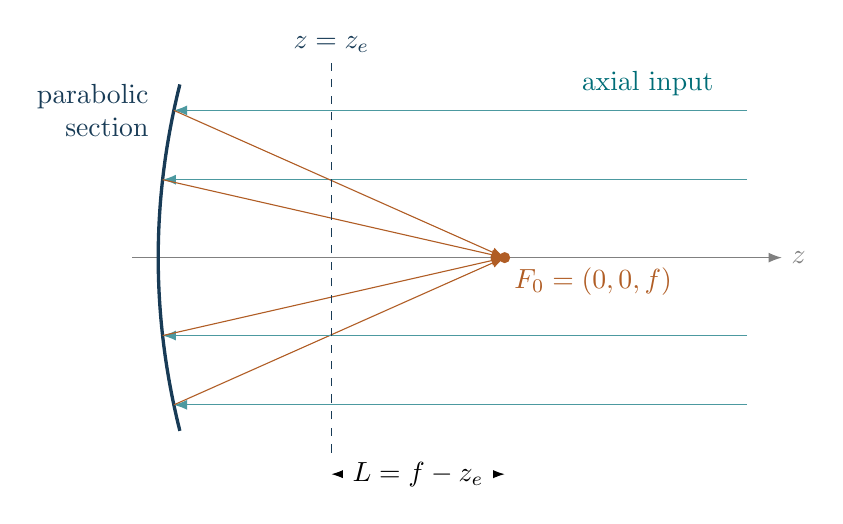
\begin{tikzpicture}[x=1.1cm,y=1.1cm,>=Latex]
 \draw[gray,->] (-.3,0)--(7.2,0) node[right] {$z$};
 \draw[ink,very thick,domain=-2:2,samples=80,variable=\r]
 plot ({\r*\r/16},{\r});
 \foreach \r in {-1.7,-.9,.9,1.7}{
  \pgfmathsetmacro{\zs}{\r*\r/16}
  \draw[accent!70,->] (6.8,\r)--(\zs,\r);
  \draw[warm,->] (\zs,\r)--(4,0);
 }
 \draw[ink,dashed] (2,-2.25)--(2,2.25);
 \node[ink,above] at (2,2.25) {$z=z_e$};
 \fill[warm] (4,0) circle (2pt) node[below right] {$F_0=(0,0,f)$};
 \node[ink,left,align=right] at (0,1.7) {parabolic\\section};
 \node[accent,above] at (5.65,1.75) {axial input};
 \draw[<->] (2,-2.5)--(4,-2.5) node[midway,fill=white] {$L=f-z_e$};
\end{tikzpicture}
\caption{Meridional geometry of the axial baseline. Horizontal distance is
$z$ and vertical distance is a transverse coordinate. The dashed plane is
a common downstream evaluation plane. The drawing is schematic.}
\end{figure}

\subsection{Surface normal and exact axial reflection}
The surface equation $G=z-(x_s^2+y_s^2)/(4f)=0$ has normal
\[
 \nabla G=(-u_s,-v_s,1),\qquad
 \vct N=\frac{(-u_s,-v_s,1)}{\sqrt{1+t}}.
\]
For $\vct d_{\rm in}=(0,0,-1)$,
$\vct d_{\rm in}\cdot\vct N=-1/\sqrt{1+t}$.
Using \eqref{eq:reflection},
\begin{equation}
 \boxed{
 \vct d_{\rm a}
 =\frac{(-2u_s,-2v_s,1-t)}{1+t}.
 }
 \label{eq:axial-reflection}
\end{equation}
Its norm is one because
$4t+(1-t)^2=(1+t)^2$. For $t<1$, it propagates along positive $z$.
Its slope is
\begin{equation}
 \vct s_{\rm a}
 =-\frac{2(u_s,v_s)}{1-t}
 =-\frac{(x_s,y_s)}{f-h}.
 \label{eq:axial-slope}
\end{equation}
Propagation from the mirror point to $z=f$ gives
$(x_s,y_s)+(f-h)\vct s_{\rm a}=(0,0)$ exactly.
Thus the ideal ray toward the axial focus has exactly the same slope:
\begin{equation}
 \boxed{\Delta\vct s=\vct0\quad\text{for axial plane-wave input}.}
\end{equation}
The actual slope itself can be large. In a meridional section,
$s_{\rm a}=-2u_s/(1-u_s^2)$, while
$s_{\rm a}\simeq-2u_s=-x_s/f$ for $|u_s|\ll1$.
The exact angle is $-2\arctan u_s$. Error remains zero in both descriptions
when each uses a consistent ideal reference.

\subsection{Independent optical-path proof of zero axial aberration}
Since $r_s^2=4fh$,
\[
 |F_0-Q_s|^2=r_s^2+(f-h)^2=(f+h)^2.
\]
For $f+h>0$, the distance is exactly $f+h$.
An incoming equal-phase plane at $z=z_{\rm in}$ contributes distance
$z_{\rm in}-h$ before reflection. The total optical path to focus is
\[
 n[(z_{\rm in}-h)+(f+h)]=n(z_{\rm in}+f),
\]
independent of footprint. This is the exact constant-phase condition.
There is no residual spherical aberration merely because $h$ or the
reflected angle is large.

\subsection{Tilt the incident wave: exact reflected direction}
Now choose the incident unit direction
\[
 \vct d_{\rm in}=(\sin\beta,0,-\cos\beta),
 \qquad |\beta|<\pi/2.
\]
Its dot product with the normal is
\[
 \vct d_{\rm in}\cdot\vct N
 =-\frac{u_s\sin\beta+\cos\beta}{\sqrt{1+t}}.
\]
Substitute into the reflection law and collect the three components:
\begin{equation}
 \boxed{
 \vct d_{\rm a}=\frac{1}{1+t}
 \begin{pmatrix}
 (1-u_s^2+v_s^2)\sin\beta-2u_s\cos\beta\\
 -2v_s(\cos\beta+u_s\sin\beta)\\
 (1-t)\cos\beta+2u_s\sin\beta
 \end{pmatrix}.}
 \label{eq:tilted-reflection}
\end{equation}
No small-angle approximation has been made. Continue with footprints
for which $d_{{\rm a},z}>0$. Define
\[
 T=\tan\beta,\qquad A=1-t.
\]
Dividing the transverse components by the longitudinal component gives
\begin{equation}
 \vct s_{\rm a}=
 \frac{\bigl(T(1-u_s^2+v_s^2)-2u_s,\,
             -2v_s(1+u_sT)\bigr)}
      {A+2u_sT}.
 \label{eq:tilted-slope}
\end{equation}
This is an exact slope, not a direction cosine and not yet an error.

In the meridional plane $y_s=0$, let $\gamma=\arctan u_s$. Since
$\sin(2\gamma)=2u_s/(1+u_s^2)$ and
$\cos(2\gamma)=(1-u_s^2)/(1+u_s^2)$,
\[
 d_{{\rm a},x}=\sin(\beta-2\gamma),\qquad
 d_{{\rm a},z}=\cos(\beta-2\gamma).
\]
Thus the signed ray angle and its slope are
\begin{equation}
 \alpha_{\rm a}=\beta-2\arctan u_s,\qquad
 s_{\rm a}=\tan\alpha_{\rm a}
 \label{eq:mirror-angle}
\end{equation}
on the forward branch. This independently checks the vector calculation.

\subsection{Specify the reference image before defining an error}
For the tilted input, choose
\begin{equation}
 F_\beta=(f\tan\beta,0,f).
 \label{eq:mirror-image}
\end{equation}
The vertex ray reflects in direction $(\sin\beta,0,\cos\beta)$ and reaches
this point on $z=f$. Therefore this choice follows the vertex ray and
removes its overall lateral displacement from the definition of error.
For a stop at the mirror, this is a natural chief-ray reference.
At small field, its image height is $f\beta$ to first order.
At finite field, \eqref{eq:mirror-image} is an explicit reference convention;
it is not a claim that every ray focuses there.

The ideal straight line from the same mirror point to $F_\beta$ has slope
\begin{equation}
 \vct s_{0,s}
 =\frac{(fT-x_s,-y_s)}{f-h}
 =\frac{(T-2u_s,-2v_s)}{A}.
 \label{eq:surface-ideal-slope}
\end{equation}
We first calculate a slope difference using this common \emph{surface}
point, denoted $\Delta\vct s_s=\vct s_{\rm a}-\vct s_{0,s}$.
We subsequently transfer the comparison to the common flat plane
required by textbook Section 4.4.

For the $x$ component, subtract the fractions:
\begin{align}
 \Delta s_{x,s}
 &=\frac{A[T(1-u_s^2+v_s^2)-2u_s]
           -(T-2u_s)(A+2u_sT)}
         {A(A+2u_sT)}\\
 &=\frac{AT(-u_s^2+v_s^2)-2u_sT^2+4u_s^2T}
         {A(A+2u_sT)}.
\end{align}
Use $4-A=3+t$ to obtain
\begin{equation}
 \boxed{\Delta s_{x,s}
 =\frac{T[(3+t)u_s^2+(1-t)v_s^2-2u_sT]}
         {(1-t)(1-t+2u_sT)}.}
 \label{eq:mirror-dsx}
\end{equation}
Similarly,
\begin{align}
 \Delta s_{y,s}
 &=\frac{-2v_s(1+u_sT)A+2v_s(A+2u_sT)}
         {A(A+2u_sT)}\\
 &=\boxed{\frac{2u_sv_sT(1+t)}
         {(1-t)(1-t+2u_sT)}}.
 \label{eq:mirror-dsy}
\end{align}
Both vanish when $\beta=0$, as required by the axial result.
They also vanish at the vertex, consistently with the chosen reference.

\subsection{Put both rays on a common flat output plane}
\label{sec:mirror-plane}
Choose a plane $z=z_e$ beyond the mirror cap under consideration and
before $z=f$. Let
\[
 L=f-z_e>0,\qquad h\leq z_e.
\]
Assume a locally single-valued ray mapping at the chosen plane.
The actual reflected ray reaches the transverse position
\begin{equation}
 \vct\xi_e=(x_e,y_e)
 =(x_s,y_s)+(z_e-h)\vct s_{\rm a}.
 \label{eq:mirror-plane-map}
\end{equation}
At this \emph{same} point, the ideal ray toward $F_\beta$ has
\begin{align}
 \vct s_{0,e}
 &=\frac{F_{\beta,\perp}-\vct\xi_e}{L},\\
 R_0&=\sqrt{L^2+|F_{\beta,\perp}-\vct\xi_e|^2},\\
 \vct q_{0,e}
 &=\frac{F_{\beta,\perp}-\vct\xi_e}{R_0}
 =\frac{\vct s_{0,e}}{\sqrt{1+|\vct s_{0,e}|^2}}.
 \label{eq:mirror-plane-reference}
\end{align}
The actual direction remains constant during free propagation, so
$\vct q_{\rm a}=(d_{{\rm a},x},d_{{\rm a},y})$ from
\eqref{eq:tilted-reflection}.
The exact error used in Section 4.4 is now
\begin{equation}
 \Delta\vct s_e
 =\vct s(\vct q_{\rm a})-\vct s(\vct q_{0,e})
 =\vct s_{\rm a}-\vct s_{0,e}.
 \label{eq:mirror-plane-ds}
\end{equation}

To relate it to the surface comparison, multiply by $L$ and substitute
\eqref{eq:mirror-plane-map}:
\begin{align}
 L\Delta\vct s_e
 &=L\vct s_{\rm a}-F_{\beta,\perp}+\vct\xi_e\\
 &=(f-h)\vct s_{\rm a}+(x_s,y_s)-F_{\beta,\perp}\\
 &=(f-h)(\vct s_{\rm a}-\vct s_{0,s}).
\end{align}
Consequently,
\begin{equation}
 \boxed{\Delta\vct s_e=\frac{f-h}{L}\Delta\vct s_s,\qquad
 \Delta\vct\xi_{\rm image}
 =L\Delta\vct s_e=(f-h)\Delta\vct s_s.}
 \label{eq:mirror-scaling}
\end{equation}
This also follows by tracing the actual ray all the way to $z=f$ and
subtracting $F_{\beta,\perp}$.

\note{The actual ray slope does not change between these planes.
The paired ideal ray changes because it must begin at the new common
point and still aim at the reference image. That is why the slope
\emph{error} at a surface point and at a flat-plane point need not be
numerically identical.}

\subsection{Recover the same result from an eikonal on that plane}
The incident plane wave has eikonal
$n(\sin\beta\,x-\cos\beta\,z)$ plus a constant.
At a mirror point, the reflected wave inherits that phase, apart from
the assumed spatially constant coating phase.
The reflected path from $z=h$ to $z=z_e$ has geometrical length
$(z_e-h)/d_{{\rm a},z}$. Therefore
\begin{equation}
 S_{\rm a}(\vct\xi_e)
 =n\left[\sin\beta\,x_s-\cos\beta\,h
        +\frac{z_e-h}{d_{{\rm a},z}}\right]+C_{\rm a}.
 \label{eq:mirror-actual-eikonal}
\end{equation}
Here $x_s,y_s$ label the ray that arrives at $\vct\xi_e$; this is a
parametric representation of an eikonal on the \emph{flat} plane.
The ideal converging wave is $S_0=C_0-nR_0$.
One convenient piston choice gives
\begin{equation}
 W_e(\vct\xi_e)
 =n\left[\sin\beta\,x_s-\cos\beta\,h
        +\frac{z_e-h}{d_{{\rm a},z}}
        +R_0-\frac{f}{\cos\beta}\right].
 \label{eq:mirror-opd}
\end{equation}
At the vertex-labelled ray,
$\vct\xi_e=(z_e\tan\beta,0)$ and
$R_0=L/\cos\beta$; hence $W_e=0$ there.
This piston choice does not affect any ray error.

The eikonal-gradient law gives
\begin{equation}
 \frac{\gradp W_e}{n}
 =\vct q_{\rm a}-\vct q_{0,e}
 \equiv\delta\vct q.
 \label{eq:mirror-opd-gradient}
\end{equation}
This is the direct bridge to Section 4.4.
If differentiating the parametric formula explicitly, the coordinate
mapping cannot be skipped. In a meridional section,
\begin{equation}
 \frac{\dd W_e}{\dd x_e}
 =\frac{\dd W_e/\dd x_s}{\dd x_e/\dd x_s}.
 \label{eq:mirror-chain}
\end{equation}
In two dimensions, the corresponding inverse-transpose Jacobian rule
was derived in Section~\ref{sec:rayerror}.
Differentiating with respect to a curved-surface coordinate and calling
it a flat-pupil gradient would yield a different, generally incorrect,
quantity.

\subsection{Small field versus small aperture: take the limits explicitly}
First let $\beta\to0$ at a fixed surface footprint. Since
$T=\beta+O(\beta^3)$, \eqref{eq:mirror-dsx}--\eqref{eq:mirror-dsy} give
\begin{align}
 \Delta s_{x,s}
 &=\beta\frac{(3+t)u_s^2+(1-t)v_s^2}{(1-t)^2}
   +O(\beta^2),\\
 \Delta s_{y,s}
 &=\beta\frac{2u_sv_s(1+t)}{(1-t)^2}
   +O(\beta^2).
 \label{eq:mirror-small-field}
\end{align}
These formulas are first order in field angle but retain finite
aperture. They need not reduce to the paraxial direction-to-slope rule.

Next suppose $|u_s|,|v_s|\ll1$ as well. Keeping the leading pupil degree
in the coefficient of $\beta$ gives
\begin{equation}
 \boxed{\Delta\vct s_s
 \simeq\beta(3u_s^2+v_s^2,\,2u_sv_s)
 =\frac{\beta}{4f^2}(3x_s^2+y_s^2,\,2x_sy_s).}
 \label{eq:mirror-primary}
\end{equation}
Multiplying by $f-h\simeq f$ gives the leading transverse image error
\begin{equation}
 \Delta\vct\xi_{\rm image}
 \simeq\frac{\beta}{4f}(3x_s^2+y_s^2,\,2x_sy_s).
\end{equation}
The pupil-quadratic, field-linear pattern is the leading coma term of
this mirror. This statement concerns only the first-order dependence
on $\beta$. Terms proportional to $\beta^2u_s$, for example, were
discarded earlier; the formula is not a complete expansion in all
pupil and field variables through total degree three.

In the meridional plane, the finite-aperture, small-field result at the
flat plane is particularly simple:
\begin{equation}
 \Delta s_e
 =\frac{f-h}{L}\,
   \beta\frac{u_s^2(3+u_s^2)}{(1-u_s^2)^2}
   +O(\beta^2).
 \label{eq:mirror-meridional-limit}
\end{equation}
It grows strongly as the outgoing rays become steep.
The exact expressions should be used when the discarded field terms
are appreciable.

\subsection{Three ways to calculate the flat-plane slope error}
For a meridional ray, put $q_{\rm a}=d_{{\rm a},x}$,
$q_0=q_{0,e,x}$, and $\delta q=q_{\rm a}-q_0=W'_e/n$.
The three results to compare are
\begin{align}
 \Delta s_{\rm exact}
 &=\frac{q_{\rm a}}{\sqrt{1-q_{\rm a}^2}}
   -\frac{q_0}{\sqrt{1-q_0^2}},\label{eq:mirror-exact-numeric}\\
 \Delta s_{\rm parax}
 &\simeq\delta q,\label{eq:mirror-parax-numeric}\\
 \Delta s_{\rm linear}
 &\simeq\frac{\delta q}{(1-q_0^2)^{3/2}}.
 \label{eq:mirror-linear-numeric}
\end{align}
The second line assumes small outgoing angles.
The third line permits a large ideal outgoing angle but linearizes in
the direction error $\delta q$.
It is the longitudinal-to-$\vct q_0$ eigenvalue of the two-dimensional
Jacobian from Section 4.4, since all rays here lie in one plane.

In the numerical comparisons below, all three formulas use the same
exact $\delta q$ from the actual and reference rays.
Thus the difference between them isolates the approximation in
\emph{converting direction error to slope error}; it does not mix in a
truncated wavefront model.

\subsection{Case A: small incident angle and small outgoing angle}
Use millimetres throughout and take
\[
 f=100\mm,\quad z_e=50\mm,\quad L=50\mm,\quad n=1,
 \qquad x_s=10\mm,\quad y_s=0,\quad\beta=10^{-4}\ \mathrm{rad}.
\]
The mirror and field parameters are
\[
 u_s=0.05,\qquad t=0.0025,\qquad h=0.25\mm,
 \qquad T=0.0001000000003333.
\]
\begin{enumerate}
 \item \textbf{Reflect the actual ray.}
 Equation~\eqref{eq:tilted-reflection} gives
 \[
 q_{\rm a}=-0.099651121696,\qquad
 d_{{\rm a},z}=0.995022438915,\qquad
 s_{\rm a}=-0.100149622560.
 \]
 \item \textbf{Locate it on the evaluation plane.}
 \[
 x_e=10+(50-0.25)(-0.100149622560)
     =5.017556277648\mm.
 \]
 The reference image height is
 $X_\beta=fT=0.0100000000333\mm$.
 \item \textbf{Construct the ideal ray from this same point.}
 \[
 s_0=\frac{X_\beta-x_e}{50}=-0.100151125552,
 \qquad
 q_0=\frac{s_0}{\sqrt{1+s_0^2}}=-0.099652602356.
 \]
 Its aperture angle has magnitude about $5.719^\circ$.
 \item \textbf{Subtract directions and slopes separately.}
 \begin{align*}
 \delta q&=1.480659945\times10^{-6},\\
 \Delta s_{\rm exact}&=1.502992456\times10^{-6},\\
 \Delta s_{\rm parax}&=1.480659945\times10^{-6},\\
 \Delta s_{\rm linear}
 &=1.015083036\,\delta q
   =1.502992792\times10^{-6}.
 \end{align*}
 \item \textbf{Convert slope error to image displacement.}
 \[
 \Delta x_{\rm image}
 =50\Delta s_{\rm exact}
 =7.514962281\times10^{-5}\mm
 =0.0751496\um.
 \]
\end{enumerate}
The paraxial result underestimates the slope error by about $1.49\%$.
The finite-angle linearization is essentially exact at the displayed
precision because the direction perturbation is very small.
For a separate small-field check,
\eqref{eq:mirror-meridional-limit} gives $1.505012531\times10^{-6}$;
also keeping only the leading pupil degree gives
$(f-h)3\beta u_s^2/L=1.49625\times10^{-6}$.
These last two values additionally approximate the mirror's field
dependence, unlike \eqref{eq:mirror-parax-numeric}.

The OPD from \eqref{eq:mirror-opd} is $W_e\simeq2.48883\nm$
at this ray. Its local derivative, rather than this single OPD value,
sets $\delta q$. The derivative with respect to $x_e$ is
$1.480659945\times10^{-6}$ for $n=1$.

\subsection{Case B: small incident angle but a large outgoing angle}
Keep the same $f,z_e,L,n,\beta$, but choose
\[
 x_s=100\mm,\qquad y_s=0,\qquad
 u_s=0.5,\qquad t=0.25,\qquad h=25\mm.
\]
This ray lies at the edge of a $200\mm$ diameter cap if that cap is used.
The small illumination angle remains $10^{-4}$ radian, yet the outgoing
ray is steep.
\begin{enumerate}
 \item \textbf{Actual reflection.}
 \[
 q_{\rm a}=-0.799939996000,\qquad
 d_{{\rm a},z}=0.600079997000,\qquad
 s_{\rm a}=-1.333055592587.
 \]
 \item \textbf{Common point on $z=50\mm$.}
 \[
 x_e=100+25s_{\rm a}=66.673610185332\mm.
 \]
 \item \textbf{Reference ray.}
 \[
 s_0=\frac{0.0100000000333-66.673610185332}{50}
    =-1.333272203706,
 \]
 \[
 q_0=-0.799986795419,\qquad
 |\alpha_0|=|\arctan s_0|\simeq53.129^\circ.
 \]
 \item \textbf{Direction and exact slope differences.}
 \[
 \delta q=4.679941922\times10^{-5},\qquad
 \Delta s_{\rm exact}=2.166111192\times10^{-4}.
 \]
 \item \textbf{Compare the approximations.}
 \begin{align*}
 \Delta s_{\rm parax}&=4.679941922\times10^{-5},\\
 (1-q_0^2)^{-3/2}&=4.629222114,\\
 \Delta s_{\rm linear}&=2.166449064\times10^{-4}.
 \end{align*}
 \item \textbf{Image displacement.}
 \[
 \Delta x_{\rm image}=50\Delta s_{\rm exact}
 =0.01083055596\mm=10.8306\um.
 \]
\end{enumerate}
The paraxial conversion is about $78.4\%$ too small.
The finite-angle linearization differs from the exact result by only
$0.0156\%$. A tiny field angle is therefore insufficient to justify
$s\simeq q$: the relevant reference aperture angle is large.

The first-order-in-field expression with exact aperture dependence,
\eqref{eq:mirror-meridional-limit}, yields
$2.166666667\times10^{-4}$, close to the exact answer.
Dropping that aperture dependence and using the leading pupil term
instead gives only $1.125\times10^{-4}$.

\subsection{Case C: finite field and finite aperture}
Keep the Case B geometry, but increase the incident angle to
$\beta=10^\circ=\pi/18$ radian. The exact formulas still apply:
\[
 T=0.176326980708,\qquad X_\beta=17.632698070846\mm.
\]
Stepwise evaluation gives
\begin{align*}
 q_{\rm a}&=-0.683657295810,
 &d_{{\rm a},z}&=0.729803193941,\\
 s_{\rm a}&=-0.936769394113,
 &x_e&=76.580765147179\mm,\\
 s_0&=-1.178961341527,
 &q_0&=-0.762614697904.
\end{align*}
The reference aperture angle is about $49.695^\circ$.
Consequently,
\begin{align*}
 \delta q&=0.078957402094,\\
 \Delta s_{\rm exact}
 &=(-0.936769394113)-(-1.178961341527)
   =0.242191947414,\\
 \Delta s_{\rm parax}&=0.078957402094,\\
 \Delta s_{\rm linear}
 &=3.694734029\,\delta q=0.291726600344,\\
 \Delta x_{\rm image}
 &=50(0.242191947414)=12.1095973707\mm.
\end{align*}
Here the paraxial result is $67.4\%$ too small and the finite-angle
linearization is $20.5\%$ too large. The second approximation now fails
because the change in direction is no longer sufficiently small for a
first-order Taylor expansion at $q_0$.
The exact slope function is needed.

\begin{table}[htbp]
\centering
\small
\setlength{\tabcolsep}{4.5pt}
\begin{tabular}{@{}lrrr@{}}
\toprule
Quantity & Case A & Case B & Case C\\
\midrule
$x_s$ (mm) & $10$ & $100$ & $100$\\
$\beta$ (rad) & $10^{-4}$ & $10^{-4}$ & $\pi/18$\\
$|\alpha_0|$ (degrees) & $5.719$ & $53.129$ & $49.695$\\
Exact $\Delta s_e$ & $1.50299\times10^{-6}$ & $2.16611\times10^{-4}$ & $0.242192$\\
Paraxial $\delta q$ & $1.48066\times10^{-6}$ & $4.67994\times10^{-5}$ & $0.0789574$\\
Finite-angle linearization & $1.50299\times10^{-6}$ & $2.16645\times10^{-4}$ & $0.291727$\\
Exact image error (mm) & $7.51496\times10^{-5}$ & $0.0108306$ & $12.1096$\\
\bottomrule
\end{tabular}
\caption{All slope differences use the same flat plane $z_e=50\mm$ and
the reference image $(f\tan\beta,0,f)$, with $f=100\mm$.
The linearization retains the exact reference aperture angle.}
\end{table}

\subsection{What this example establishes}
The axial paraboloid has zero slope error, even for steep rays.
Tilting its illumination introduces a footprint-dependent error.
The wavefront and reflection calculations agree through
$\gradp W/n=\delta\vct q$ on the common plane.
Case A supports the paraxial conversion; Case B requires the finite-angle
Jacobian; Case C requires the exact slope difference.

\caution{A slope difference $\Delta s$ is dimensionless, and it is
approximately an angular error only in the paraxial limit.
The actual angular error in a meridional plane is
$\Delta\alpha=\arctan s_{\rm a}-\arctan s_0$ on a consistent branch.
The transverse ray error is the length $L\Delta s$.
These three quantities answer different questions.}

\end{document}
